\section{Review reporting}
\subsection{Primary motivation for developers contributing in open source}
The main purpose of this study is to find the movitvation of developers contributing in OSS project. For each selected study, I analyzed any motivation reported that was empirically identified or evaluated.

\subsubsection{Intrinsic motivations}
Our exploration of developer motivation in open-source software (OSS) projects begins with intrinsic motivations, the internal drivers that fuel participation for personal satisfaction rather than external rewards. This encompasses a broad spectrum of factors, including: play value, the inherent enjoyment derived from the coding process; community engagement, the sense of belonging and collaboration found within OSS projects; learning, the opportunity to develop new skills and expand technical knowledge; personal interest, the desire to work on projects that align with individual passions; altruism and ideology, the belief in contributing to a greater good and supporting the open-source philosophy; need for autonomy, the freedom to work independently and creatively; and reciprocity/introjected regulation, the desire to contribute back to the community and maintain a sense of personal responsibility for the project's success. I will delve deeper into each of these intrinsic motivations in the following sections, examining their unique influence on developer behavior within the OSS landscape.

1. Play value

In contrast to traditional software development, which often prioritizes external rewards like monetary compensation and career advancement, OSS projects offer a unique space where play value emerges as a central driving force. Play value, in this context, encapsulates the inherent enjoyment, intellectual stimulation, and creative fulfillment developers experience through the act of programming and problem-solving \parencite{05bitzer2007intrinsic, 06ye2003toward, 08zhang2024paid, 09lakhani2005hackers, 11gerosa2021shifting, 12choi2015characteristics,13li2012leadership,16ke2008motivations,17alexander2002working, 18oreg2008exploring}. Let's examine why this is such a powerful motivator.

For many developers, OSS represents a playground for experimentation and innovation. Unburdened by strict commercial deadlines or rigid specifications, they are free to explore novel ideas, test unconventional approaches, and engage in the iterative process of building software purely for the intrinsic satisfaction it provides .  The act of turning concepts into functional code can be deeply rewarding.

OSS communities often tackle complex technical problems that demand creative solutions.  Developers who are drawn to intrinsically motivating challenges revel in the opportunity to dissect intricate issues, devise elegant workarounds, and optimize code performance. This continuous learning process creates a sense of mastery and accomplishment that fuels further engagement.

Commercial software development typically necessitates compromises – feature trade-offs, adherence to proprietary standards, and prioritization of market demands over pure technical curiosity. In contrast, OSS projects offer developers a liberating space to exercise their technical creativity without external pressures. This autonomy nourishes problem-solving and innovation for its own sake.

The collaborative aspect of OSS can itself be a form of play.  Engaging with fellow developers, brainstorming solutions, exchanging knowledge, and contributing to a shared creation can be intellectually stimulating and enjoyable. This camaraderie fosters a playful sense of experimentation and discovery within the community.


2. Community engagement

The act of conceptualizing the open-source community as a metaphorical family, united in pursuit of shared objectives, can be a powerful catalyst for developer participation \parencite{05bitzer2007intrinsic,07zhao2024openrank, 08zhang2024paid, 09lakhani2005hackers, 13li2012leadership, 16ke2008motivations, 17alexander2002working}. This collaborative environment fosters contributions aimed at communal advancement, even when they may not yield immediate personal gain for the individual developer. Participation in open-source projects can be fueled by a profound sense of belonging and an alignment of personal values with those of project teams and the open-source movement at large.

The chart \ref{fig:motivationDimension} underscores the complex interplay of motivations that drive developer participation in open-source projects. While social factors are paramount, career considerations and political beliefs also play a significant role. This diversity of motivations highlights the need for a nuanced understanding of the open-source community and tailored strategies to attract and retain developers.

\begin{figure}[ht]
    \centering
    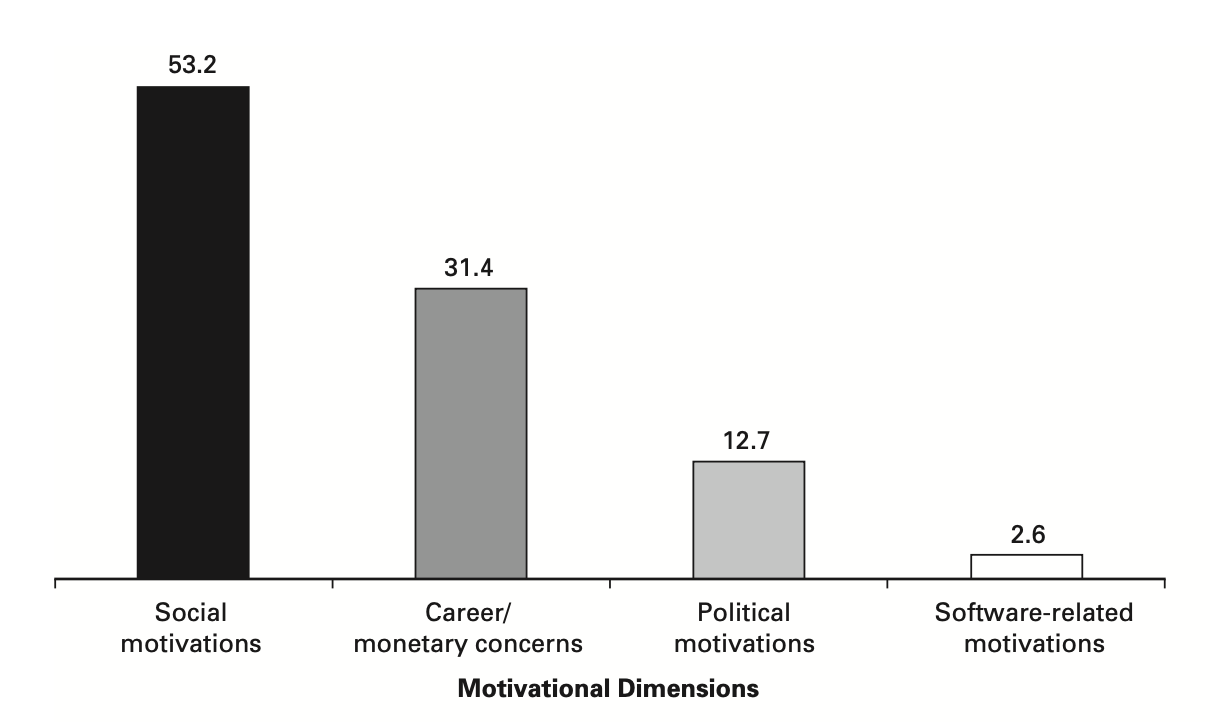
\includegraphics[width=0.7\linewidth]{figs/motivationDimension.png}
    \caption{As a proportion of all contributors to OSS, developers by motivation class \cite{ghosh2002free}}
    \label{fig:motivationDimension}
\end{figure}

Additionally,  a conviction regarding the inherent value of open-source code, paired with a perceived responsibility to contribute to the free and OSS ecosystem, serves as a significant motivator for developers. Cultivating a sense of belonging and fostering a shared purpose within the community or project team can thus be instrumental in empowering individuals to become active participants and contributors in the open-source software development landscape.



3. Learning

Research consistently identifies learning as a primary impetus for individuals to actively engage in OSS communities \parencite{06ye2003toward, 07zhao2024openrank, 08zhang2024paid, 09lakhani2005hackers, 10wu2007empirical, 11gerosa2021shifting, 12choi2015characteristics, 17alexander2002working, 18oreg2008exploring}. OSS projects present multifaceted learning environments; developers are drawn to the inherent opportunities to acquire knowledge from the systems themselves, to collaborate and gain insights from fellow community members, and to reciprocally disseminate their own expertise.

Participation within OSS communities extends beyond the purely technical exchange of knowledge, encompassing a rich social dimension. By directly engaging in open-source projects, developers immerse themselves in a collaborative network of peers, often spanning skill levels and expertise. This fosters a dynamic learning ecosystem where individuals benefit from informal mentorship opportunities, observing problem-solving approaches employed by more experienced contributors, and receiving constructive feedback that accelerates their professional growth.

Moreover, the act of contributing to a shared knowledge base empowers developers and reinforces self-efficacy. The potential for continuous self-development, the pursuit of mastery, and the ability to give back to a community dedicated to knowledge-sharing serve as profound and enduring sources of motivation for many software contributors.

4. Personal interest

The concept of the "personal itch," as articulated by Eric S. Raymond, illuminates a key motivator for developer participation in OSS projects. Individuals often engage in OSS development to address a specific problem or augment functionality that directly aligns with their personal or professional needs. The desire to create a solution that may not otherwise exist, driven by this personal necessity, serves as a potent catalyst for engagement.

Furthermore, the inherent intellectual challenge of solving complex programming problems stands as a significant motivator for developers seeking to contribute to open-source initiatives. The opportunity to grapple with intricate coding puzzles, apply problem-solving strategies, and ultimately contribute to the solution can be deeply fulfilling for those driven by a passion for programming.

The sense of creativity fostered within the OSS landscape is another powerful draw. Developers are empowered to express their ingenuity, explore innovative solutions, and continuously hone their skills through the development of tools or solutions that serve their own requirements or those related to their work. This blend of personal utility, creative expression, and continuous learning establishes a compelling environment that attracts and sustains developer involvement.

5. Altruism and ideology

OSS development thrives in part due to the contributions of individuals motivated by altruism and ideological convictions. This section explores these factors and their influence on developer participation. A significant driver for many developers is the inherent satisfaction derived from assisting others. Contributing to open-source projects allows them to directly improve software used by a wider community. This collaborative environment fosters a sense of purpose, as developers witness the positive impact of their work on others

Many developers are drawn to  the core principles of open-source software, including transparency, collaboration, and the democratization of technology. Participation allows them to contribute to a development model that emphasizes open access and fosters a sense of community.  Additionally, developers can be motivated by a desire to create software that benefits the greater good by being freely available and readily modifiable. This aligns with their altruistic desire to contribute to society and maintain strong social bonds.

Altruism and ideological alignment with open-source principles play a vital role in propelling developer participation. Both the satisfaction of helping others and the commitment to open-source ideals create a compelling environment that attracts and retains developers within the OSS ecosystem.

6. Autonomy

The open-source software environment provides a platform where developers can exercise a high degree of autonomy, making it particularly attractive to those valuing self-determination. The ability to select projects of interest, dictate their involvement, and contribute independently fulfills the intrinsic need for autonomy. This freedom to innovate and pursue solutions without rigid constraints becomes a compelling motivator, drawing developers who seek a sense of control and ownership over their contributions.

Unlike traditional software development environments that might be constrained by rigid hierarchies or top-down management styles, the open-source model empowers developers to chart their own path. They can choose to focus on areas that align with their passions, explore new technologies, or experiment with novel approaches without the need for constant external approval.  This sense of agency and self-direction is deeply fulfilling for those who thrive in environments where their initiative and creativity are valued.

7. Reciprocity and introjected regulation

Open-source communities thrive on a powerful sense of reciprocity. Developers who have directly benefited from freely available open-source software often feel a deep-seated obligation to give back, fueling their participation and ensuring the continued growth of the ecosystem. This desire to repay the community for the invaluable resources they've received becomes a motivating force.

Additionally, introjected regulation plays a role in influencing developer behavior. The internalization of expectations can lead to feelings of pride, guilt, or shame regarding contributions to open-source projects. This desire to maintain a positive self-image, live up to personal standards, and avoid negative emotions can significantly drive participation as developers strive to meet both their own expectations and those they perceive the community holds.

\subsubsection{Extrinsic motivations}

Beyond the intrinsic factors explored in the previous chapter, extrinsic motivations also play a significant role in driving developer participation in open-source projects. This chapter delves into these external factors, including the potential for signaling skills and experience to potential employers, garnering recognition and building reputation within the open-source community, and potentially obtaining external rewards such as monetary compensation or job opportunities.

I will also examine how extrinsic motivators can intersect with a developer's  desire to improve software quality. Contributions to high-profile projects can serve as a powerful signal of competence, while active participation may lead to opportunities to collaborate with skilled developers and gain valuable experience.  Furthermore, I will explore the concept of role transformation: how continued involvement in the open-source landscape can elevate a developer's standing, potentially opening doors to leadership roles, consulting positions, or  job offers within companies heavily invested in open-source technologies.

1. Signaling and recognition

Participating in OSS projects allows developers to publicly showcase their abilities and commitment. Within the highly competitive software development field,  OSS contributions provide concrete evidence of a developer's abilities, enhancing their reputation and potentially unlocking new opportunities.  Open-source involvement demonstrates not only technical skills but also a dedication to the broader community and a drive for innovation.

Open-source projects offer developers a platform to display their talents to potential employers, boosting their professional standing. Unlike traditional resumes or interviews that provide a more limited view, OSS contributions offer real-world proof of a developer's capabilities. Employers often see active participation as indicative of both technical skill and the ability to collaborate effectively in a team setting.

The recognition garnered from fellow developers within the open-source community serves as a powerful motivator. The open-source model promotes collaboration, transparency, and continuous improvement, resulting in a space where contributions are acknowledged and celebrated. This validation from peers acts as a potent incentive for developers to further advance their skills and continue making meaningful contributions to projects they're passionate about.

Active engagement in open-source projects supports developers in building strong reputations within their field, positioning them as experts in their niche. Through consistent, high-quality contributions, thoughtful insights, and constructive participation, developers gain respect within the community. This recognition elevates their professional stature and fosters new possibilities for collaboration, networking, and career progression. Ultimately, leveraging their open-source work as a showcase is beneficial not only to the individual developer but also contributes to the advancement of the entire developer community.

2. Improving software quality

Some developers engage in open-source projects to create high-quality software that is accessible to a wider audience and can benefit the community. Open-source development fosters a collaborative environment where developers from diverse backgrounds come together to share their expertise and work towards common goals. By leveraging the collective intelligence and resources of the community, developers can create software that is not only robust and reliable but also tailored to address the evolving needs of users across different industries and domains. This democratization of software development ensures that innovative solutions are not confined to proprietary ecosystems but are freely available for anyone to use, modify, and redistribute.

By participating in open-source projects, developers can access and contribute to software that meets their specific needs and preferences, often surpassing proprietary alternatives. Unlike closed-source software, which may be limited by proprietary restrictions and licensing fees, open-source projects offer greater flexibility and transparency. Developers have the freedom to inspect, modify, and enhance the code according to their requirements, empowering them to create customized solutions that are more efficient, secure, and adaptable. This collaborative and iterative approach to software development not only fosters innovation but also fosters a sense of ownership and pride among contributors, who are motivated by the collective impact of their efforts on the broader community.

3. External rewards

While publicly discussions often prioritize the significance of intrinsic motivations, extrinsic rewards such as promotions, financial incentives, increased compensation, and professional advancement remain potent drivers of developer participation in open-source projects. Tangible rewards hold substantial appeal, particularly for those who utilize open-source involvement as a strategic tool for career development and financial gain. Within a highly competitive labor market emphasizing demonstrable skills and practical experience, active open-source contributions tangibly augment a developer's professional credentials and enhance their overall marketability.

Developers may be drawn by the potential financial returns derived from open-source participation, such as new job opportunities or consulting contracts. By establishing a visible record of expertise and successful contributions, developers attract the attention of companies or clients who value their skills, potentially leading to lucrative positions. Beyond traditional employment, open-source involvement can serve as a foundation for supplementary income streams, such as consulting services, training workshops, or speaking engagements, which cultivate both financial rewards and professional recognition.

Furthermore, the pursuit of career advancement and professional distinction strongly motivates developers to engage with open-source projects. Establishing oneself as a thought leader or subject matter expert within the community cultivates opportunities for leadership positions, mentorship roles, or invitations to esteemed conferences and industry events.  The visibility and reputation fostered through such contributions heighten a developer's standing and create new pathways for professional growth and development.  Ultimately, while intrinsic motivations undeniably fuel enthusiasm and dedication,  extrinsic rewards remain indispensable in attracting and sustaining long-term participation in open-source initiatives.

A study examining the dynamics of paid and volunteer open-source developers within the Rust project has revealed significant disparities in their contribution behaviors \cite{08zhang2024paid}. Notably, core developers who receive compensation demonstrate a higher frequency of contributions compared to volunteers \ref{fig:contribution_frequency}. This suggests that financial incentives may play a role in driving sustained engagement.

\begin{figure}[ht]
    \centering
    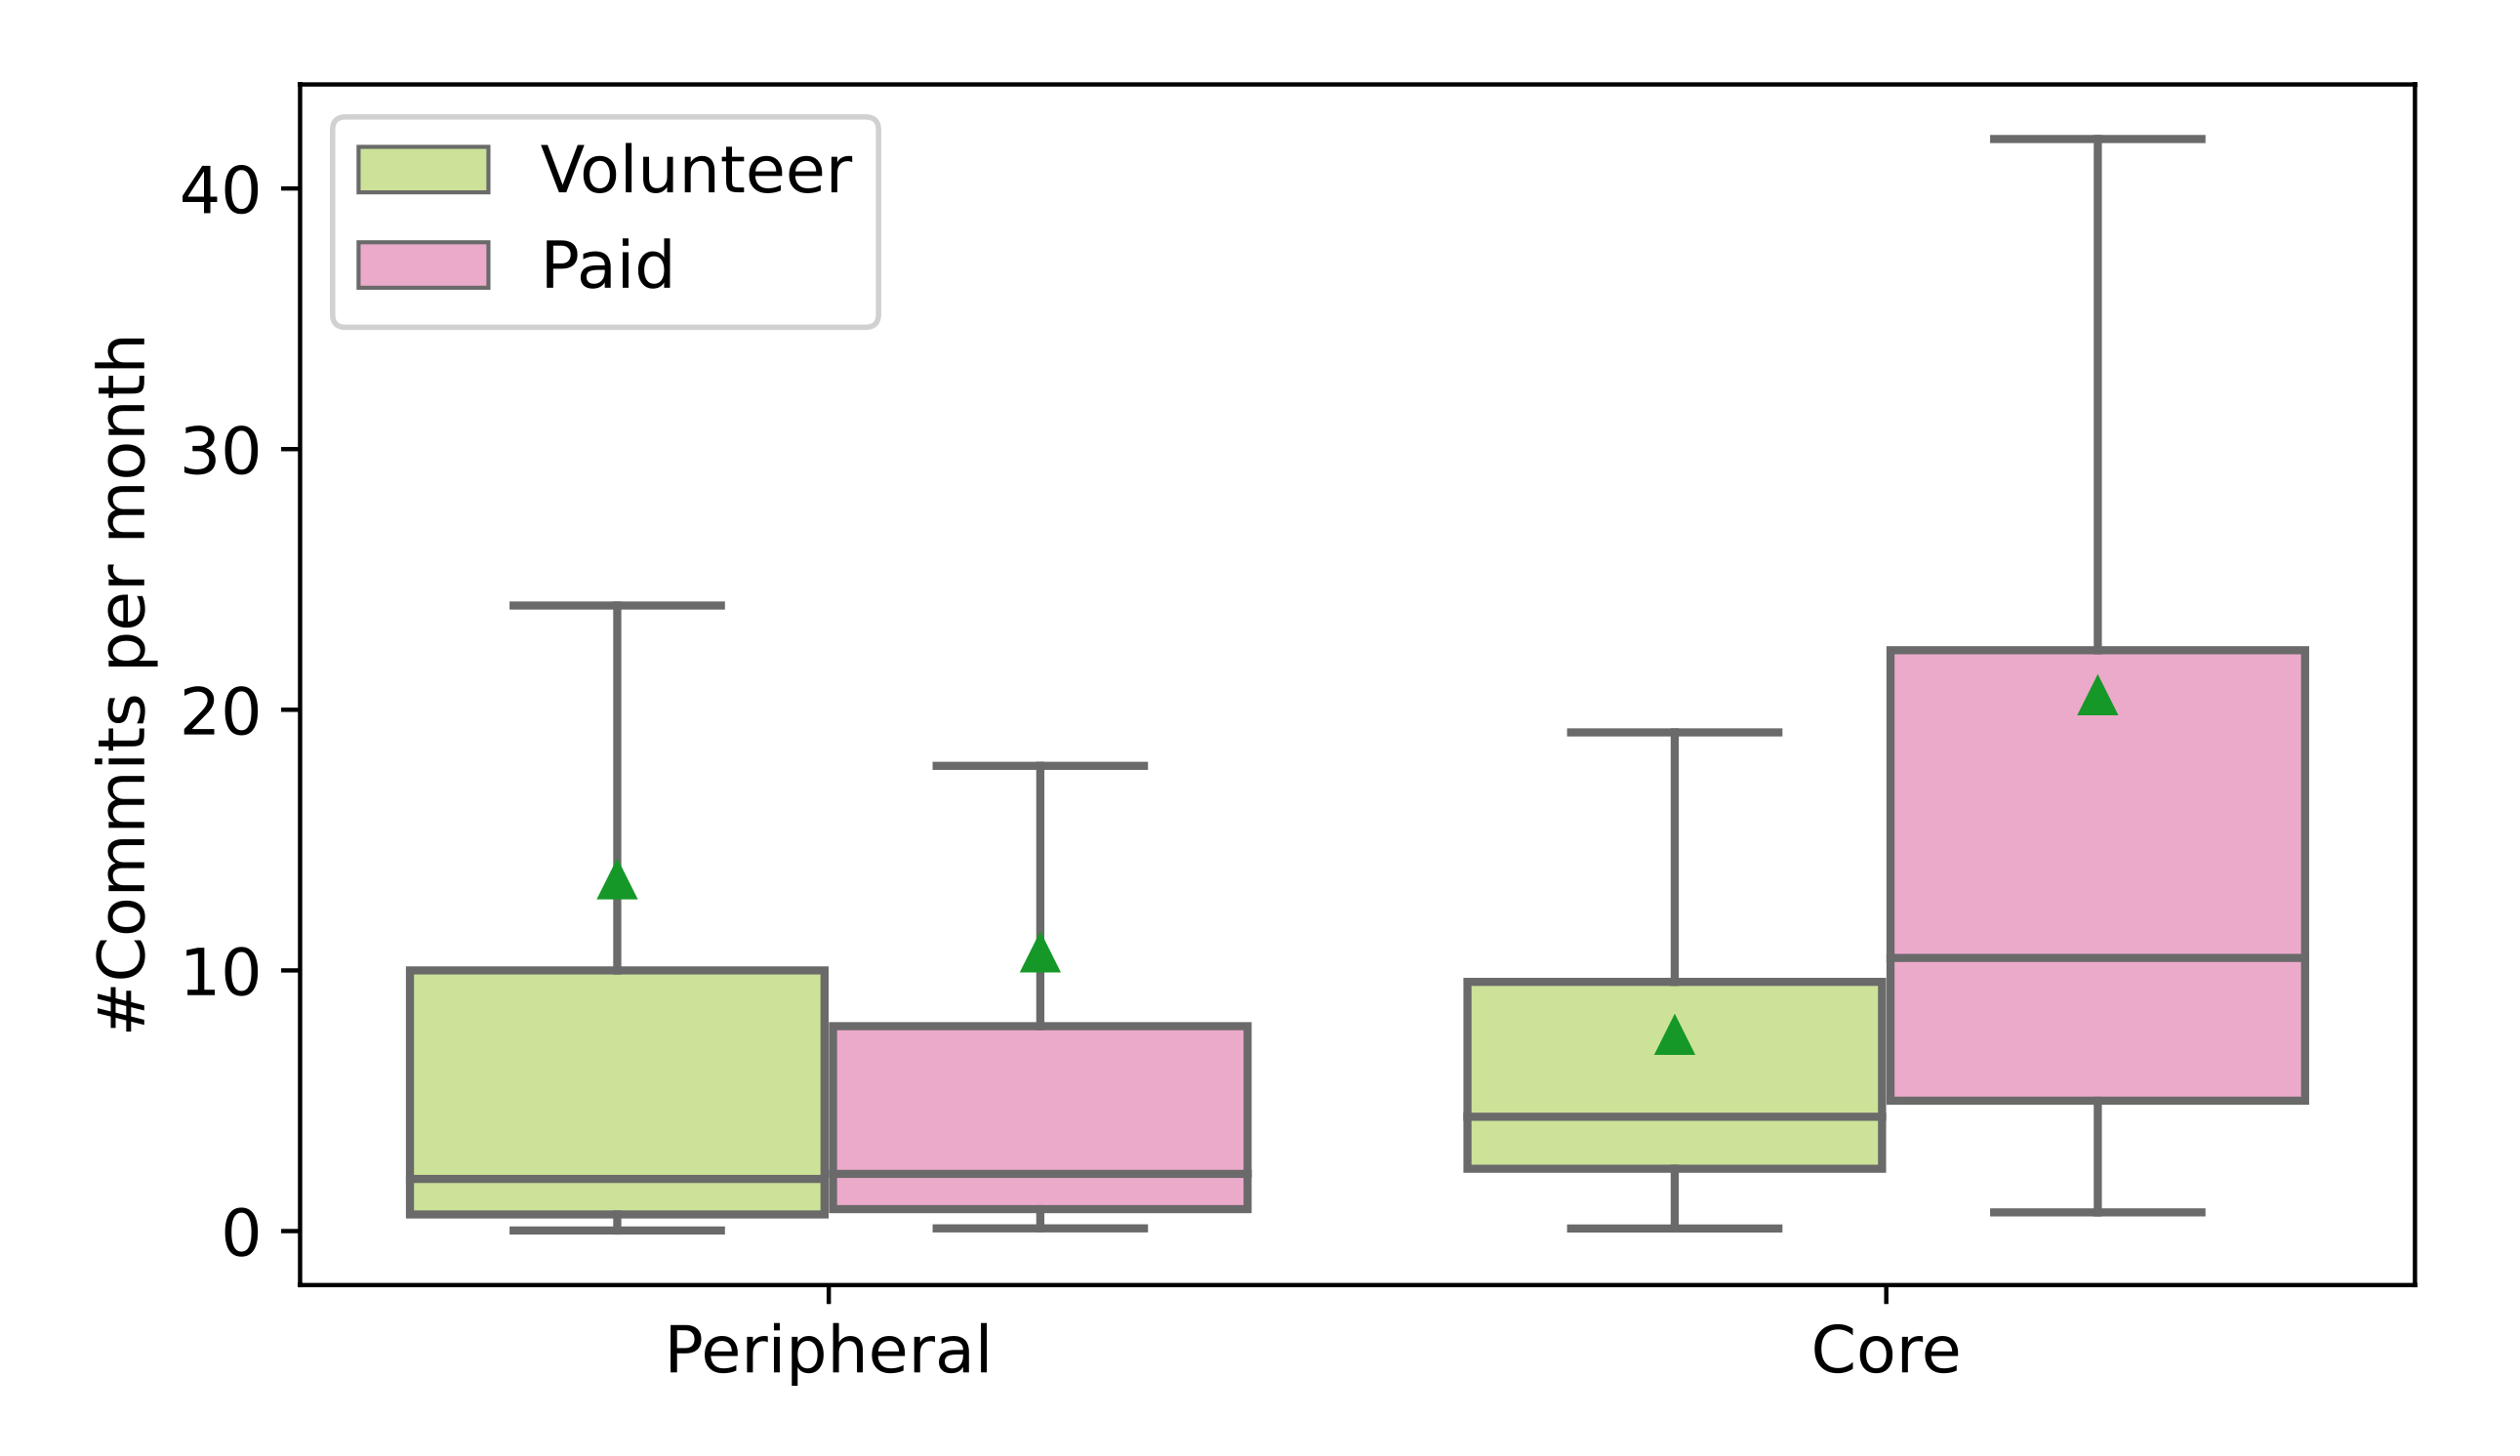
\includegraphics[width=0.65\linewidth]{figs/Contribution_frequency.png}
    \caption{How often paid and volunteer developers contribute to Rust project \cite{08zhang2024paid}}
    \label{fig:contribution_frequency}
\end{figure}


Moreover, commits from one-time paid developers tend to be larger in scope, potentially encompassing more impactful code changes than those of one-time volunteers. This highlights a possible correlation between compensation and the magnitude of contributions. Peripheral paid developers exhibit a higher inclination towards implementing new features compared to unpaid contributors. This trend underscores how financial incentives might influence not only the quantity but also the innovative nature of contributions within the open-source ecosystem.

Collectively, these findings illustrate the complex dynamics of mixed-motivation OSS projects. Understanding these distinctions is crucial for project maintainers seeking to effectively leverage the collaborative potential of both paid and volunteer contributors, ultimately strengthening the sustainability of OSS projects.

4. Role transformation

One of the defining characteristics of OSS projects is the transformation of roles.  Unlike traditional software development models, where users and developers occupy distinct positions, OSS communities blur these lines.  Anyone, from seasoned developers to individuals with technical curiosity, can become a contributor.  This inclusive nature fosters a sense of ownership and empowers users to actively shape the project's evolution.  The potential to transition from user to developer offers a compelling incentive for participation, fostering a community where everyone's voice is valued, and diverse perspectives are encouraged.

Furthermore, the ability to directly address user needs serves as a significant motivator for developers to contribute to open-source projects.  Whether these needs arise from professional or personal endeavors, developers within the OSS community are driven by the desire to create software that solves real-world problems and enhances the user experience.  This direct connection between developers and users fosters a collaborative environment where both parties benefit from the shared knowledge and dedication to continuous improvement.

\subsection{Impact of social dynamics}

In addition to investigating the motivations of developers, this research also examined the significant influence of social dynamics on the participation of developers in open-source projects. Through a comprehensive analysis of 13 pertinent studies selected from a pool of over 20 papers, this research has yielded several key findings. These findings highlight the multifaceted nature of developer engagement in open-source initiatives and underscore the importance of social interactions in shaping participation patterns. The subsequent sections will elaborate on these findings, providing a nuanced understanding of the interplay between individual motivations and social forces within the open-source software development ecosystem.

\subsubsection{Community interaction}
The level of interaction within an open-source community is a significant determinant of developer participation. Active communication channels, encompassing forums, mailing lists, and chat platforms, provide essential avenues for collaboration, knowledge sharing, and mutual assistance. These interactions foster a sense of community and belonging, encouraging developers to actively engage with the project and contribute their expertise. Conversely, projects with limited or ineffective communication channels may struggle to attract and retain contributors, as developers may feel isolated or lack the necessary support to make meaningful contributions.


Empirical research consistently demonstrates that developers derive substantial satisfaction from collaborative endeavors and the opportunity to assist others within the open-source ecosystem. Collaboration and teamwork are not merely instrumental means to achieve project goals but are also intrinsically rewarding for developers. The sense of community engendered by open-source projects, along with the opportunity to interact with peers and contribute to a shared endeavor, are integral to the ethos of open-source software development.

The establishment of robust communication infrastructure and feedback mechanisms is paramount for sustaining active developer participation. Clear, transparent, and efficient communication facilitates the resolution of technical issues, the exchange of innovative ideas, and the coordination of efforts among team members. Moreover, constructive feedback loops enable developers to learn from each other, refine their skills, and enhance the quality of their contributions. Cultivating a supportive and communicative environment fosters a sense of camaraderie and shared purpose, thereby augmenting developer engagement and productivity.

The integration of social features within open-source platforms, such as mechanisms for connecting individuals seeking assistance with those willing to provide it, can substantially enhance community interactions and support. The open-source ethos is intrinsically predicated on collaboration and the open exchange of knowledge, and social platforms facilitate these interactions by creating virtual spaces for developers to connect, communicate, and collaborate. The sense of belonging to a community of like-minded individuals fosters camaraderie, mutual assistance, and a shared sense of purpose, all of which contribute to sustained engagement and project success.

The presence of experienced developers who are willing to mentor newcomers is a crucial catalyst for promoting participation and retention within open-source communities. Mentorship programs provide novice developers with invaluable guidance, support, and encouragement, empowering them to overcome challenges, acquire new skills, and integrate seamlessly into the community. This intergenerational transfer of knowledge is essential for the long-term sustainability and growth of open-source projects. By fostering a welcoming and inclusive environment that values mentorship and knowledge sharing, open-source communities can attract and retain a diverse range of contributors, ensuring the continued vitality and innovation of the open-source software ecosystem.




\subsubsection{Networking opportunities}
Novice contributors often transition their initial motivations towards career-oriented goals, leveraging open-source projects as a portfolio to showcase their skills to potential employers \cite{05bitzer2007intrinsic,11gerosa2021shifting}. Participation in these projects offers invaluable networking opportunities, fostering connections with industry professionals and paving the way for career advancement \cite{10wu2007empirical,11gerosa2021shifting,13li2012leadership}. By demonstrating their expertise and building a reputation within the open-source community, developers can attract job offers, consulting opportunities, and further professional development. Moreover, the open-source environment allows developers to gain experience with diverse technologies, tools, and methodologies, broadening their skillset and making them more adaptable to the evolving demands of the tech industry.

Open-source projects serve as a platform for developers to connect with industry peers, experts, and potential employers \cite{10wu2007empirical,11gerosa2021shifting,13li2012leadership}. These connections can lead to collaborations on new projects, expanding professional networks and opening doors to career growth opportunities. The collaborative nature of open-source projects allows developers to establish relationships with like-minded individuals, fostering a supportive community that encourages knowledge sharing and mutual growth.  Additionally, engaging with established open-source communities can provide developers with exposure to industry best practices, coding standards, and project management methodologies, further enhancing their professional capabilities.

Open-source projects are inherently collaborative environments, providing developers with ample opportunities to share knowledge, learn from others, and enhance their skills. The exchange of ideas, feedback on code, and exposure to diverse perspectives within the community foster continuous learning and skill improvement. Through interactions with other developers, mentorship, and exposure to new ideas and technologies, developers are motivated to stay engaged and contribute to the project's ongoing success \cite{05bitzer2007intrinsic,06ye2003toward,09lakhani2005hackers,13li2012leadership}. This culture of continuous learning and knowledge sharing also helps developers stay abreast of the latest trends and innovations in the tech industry, ensuring their skills remain relevant and in demand.


\subsubsection{Community culture and support }

Engaged and supportive open-source communities act as a catalyst for developer contributions by offering assistance, constructive feedback, and a sense of belonging. This collaborative atmosphere nurtures knowledge sharing, mutual support, and a strong sense of community among developers. Ultimately, positive social interactions and a supportive environment within these communities drive increased motivation and sustained engagement among developers. \cite{10wu2007empirical,12choi2015characteristics,13li2012leadership,16ke2008motivations}.

Social coding platforms have revolutionized the open-source landscape, shifting the culture from its traditional hacker-centric roots to a more inclusive, collaborative community. By lowering barriers to entry, these platforms have made open-source projects more accessible and welcoming to newcomers, regardless of their technical expertise \cite{06ye2003toward,11gerosa2021shifting}. They foster a sense of belonging and encourage participation through features like issue tracking, discussion forums, and code review tools, promoting knowledge sharing and collaborative problem-solving. This cultural shift has not only broadened the pool of contributors but has also led to more diverse perspectives and innovative solutions within the open-source ecosystem.

Roles within OSS communities are dynamic and fluid, allowing members to assume greater responsibilities by contributing meaningfully to projects. As individuals transition between roles, they actively influence the social dynamics and structure of the community, ultimately driving its evolution \cite{06ye2003toward}. This flexibility enables OSS communities to adapt and thrive in response to the evolving needs of projects and the diverse contributions of their members.


Open-source platforms that promote collaboration and offer diverse avenues for appreciation, ranging from formal accolades to informal gestures like awarding stars to projects, significantly enhance the sense of belonging and recognition among community members. Active engagement in these communities allows developers to gain recognition for their contributions, cultivate a positive reputation, and establish a personal brand within the wider developer community \cite{11gerosa2021shifting,13li2012leadership}.

The paper "OpenRank Leaderboard: Motivating Open Source Collaborations Through Social Network Evaluation in Alibaba" presents a study conducted to explore the impact of the OpenRank Leaderboard on open source collaborations within Alibaba's projects \cite{07zhao2024openrank}. The research methodology involved a mixed-methods approach, including case studies, surveys, analysis of project metrics data, semi-structured interviews, and thematic coding. The study focused on seven open source projects initiated by Alibaba, aiming to investigate how gamified leaderboards can motivate collaboration and drive innovation in software development.

\begin{figure}[ht]
    \centering
    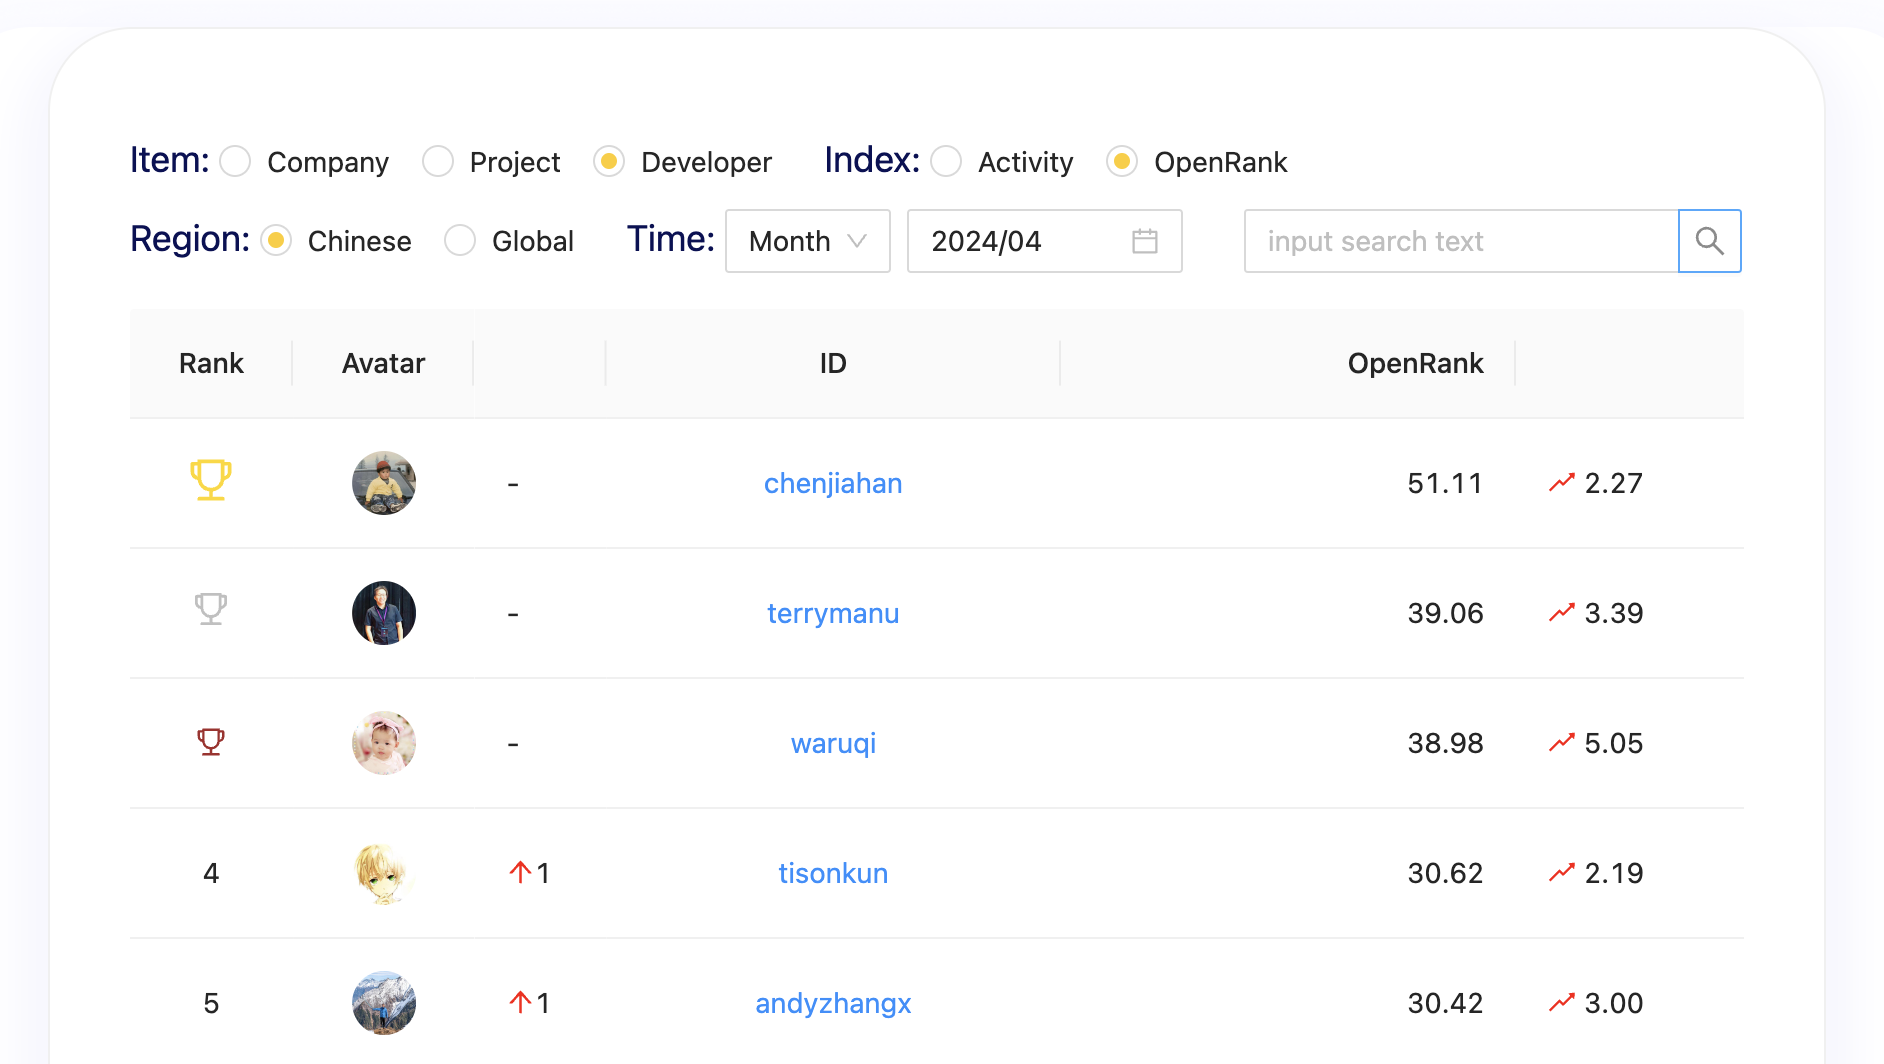
\includegraphics[width=0.85\linewidth]{figs/openrank.png}
    \caption{A screenshot of the interface of the OpenRank Leaderboard in May, 2024}
    \label{fig:openrank}
\end{figure}



Through the implementation of the OpenRank Leaderboard, the study found that developers were motivated to engage in more transparent communication, leading to improved collaboration behavior and a better community atmosphere. The leaderboard incentivized developers to make smaller, independent \ac{pr} and avoid direct commits to the repository, ultimately enhancing the quality of code contributions and fostering continuous improvement within the projects. The research also highlighted the role of the leaderboard in promoting healthy competition among developers, encouraging sustained engagement, and driving innovation within the open source projects.

The findings of the study indicated that the OpenRank Leaderboard effectively evaluates and steers developers' contributions, leading to positive behavioral changes and enhanced collaboration habits. Developers expressed a favorable perception of using graph network algorithms for contribution evaluation, with many acknowledging the alignment of rankings with their community perceptions and the value of combining results with community incentive operations. Overall, the study contributes valuable insights into the impacts and perceptions of using leaderboards as a gamification mechanism in company-led open source projects, emphasizing the importance of social network evaluation in motivating open source collaborations and driving innovation in software development.


\subsection{Contribution barriers}



\clearpage